\documentclass[10pt,a4paper]{report}
\usepackage[utf8]{inputenc}
\usepackage{amsmath}
\usepackage{amsfonts}
\usepackage{wrapfig}
\usepackage{subfig}
\usepackage{amssymb}
\usepackage{makeidx}
\usepackage{graphicx}
\usepackage[a4paper,margin=1in]{geometry}
\author{Erik Rosvall \\ Sven Hermans}
\title{Text Based Information Retrieval \\ Visual Question Answering Project \\ Part 1 \& 2}
\begin{document}
	\maketitle
	\section*{Part 1 - Resubmission}
		Part 1 of the assignment had to be redone in a significant way, and many parts of the previously submitted code are no longer used. That model was to simplistic and therefore resulted in poor prediction performance. The report will explain how and where the changes were made.
	\subsection*{Preprocessing}
		The preprocessing has changed from a one-hot representation to an embedding layer. While a one-hot representation should in theory work well, we found that using the embedding performs similarly, but simplifies the interactions and code in general for the program. We still did a conversion to index form with the help of a vocabulary dictionary, but the last step of the preprocessing step changed. We still used padding to enable batch computing. This had some effects on the accuracy calculations, but is necessary for such a deep architecture.
	\subsection*{Autoencoder}
		\begin{wrapfigure}{r}{0.5\textwidth}
		\begin{center}
			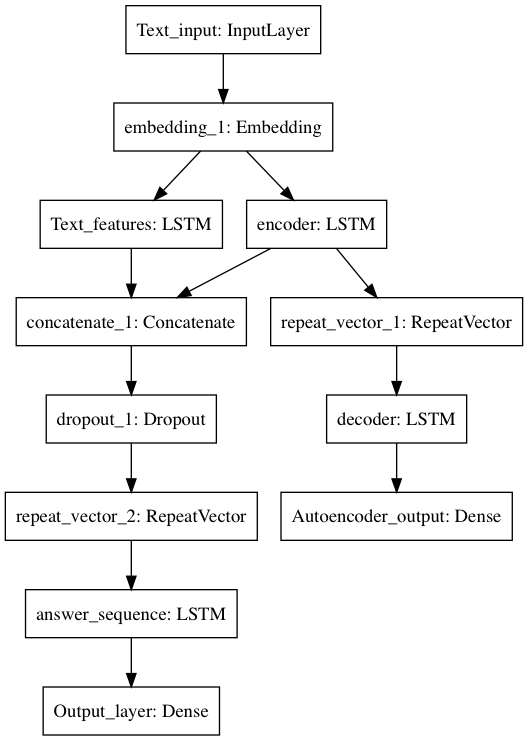
\includegraphics[width=0.3\textwidth]{text_classifier_w_autoencoder.png}
		\end{center}
		\caption{Model architecture for the text based question answering. \label{text_classifier_w_autoencoder}}
	\end{wrapfigure}
	Instead of using a stacked, many-to-many autoencoder, we changed the autoencoder to a single layer with one-to-one representation. This in order to try to force the model to learn a more non-linear representation to use in the prediction task. The very good results regarding the autoencoder in the previous report were likely due to the parameter \texttt{return\_sequence = True} which allows the model to learn a simple semi-linear representation between the steps. In this version however, we're not reducing the dimensionality of the data to the same degree, now settling for 512 rather than 50 from before.


	As seen in figure \ref{text_classifier_w_autoencoder} we've chosen an integrated structure, with a single input and embedding layer, that then outputs to both a normal LSTM layer for feature extraction and one for lower dimension encoder. These two models are evaluated separately, but trained simultaneously. The encoder and LSTM feature extraction are then concatenated and fed into an answering LSTM. The Dense layers are there to aid output with \texttt{softmax} activation function. The Dropout is to try to limit overfitting, something that the literature referenced as a problem for LSTM networks.
	
	Training the new autoencoder with $ 100 $ epochs results in an accuracy of $ 81.2 \%$ for the test data.  An example of the output (\textit{oov} stands for Out of Vocabulary):
	\\\textit{what is behind the plastic bag in the $ < $oov-token$ > $
	\\ what is behind the ironing board in the image322  }

	\subsection*{Prediction results}
	The predicted answers reach an accuracy of $ 18.9 \% $ and a\textit{WUPS} score of  $ 0.203 $. Since we're dealing with multiple possible answers there is ambiguity of how to calculate accuracy. We used the mean fraction of correctly classified words for each question.


\pagebreak



	\section*{Part 2}
	Many features stay the same between the text-only prediction from part 1 and the addition of visual data. The layers "behind" the concatenation layer don't change. The decoder and autoencoder output also stay the same between the old model and the new one.
	\subsection*{Inclusion of visual features}
	We decided to add the visual features after extracting the text features. We could have chosen to concatenate the text feature vector with the visual one, but we felt that the model became less modular and the fact that we used a specific LSTM layer for prediction negated the need to blend these two features. It also kept the text-only model and visual one as close as possible. 
	\subsection*{Inclusion or exclusion of autoencoder}
	When considering the performance of the model, the need for the extra complexity and training time of the autoencoder were discussed and compared. The two models can be seen in figure \ref{vqa}. The features extracted by both the encoder and \texttt{Text\_features}-layer should (in theory) be able to learn independent features of the text, trying to ignore things like grammatical quirks and non informative words (like \textit{the} etc) to keep the defining words or features. One of the problems with neural networks in general is the difficulty to interpret what that representation is, but if the encoder for example is able to reconstruct the sentence well the information has been condensed to a more informative state.
	\begin{figure}[h]
		\centering
		\begin{tabular}{ c | c }
			\subfloat[Full model]{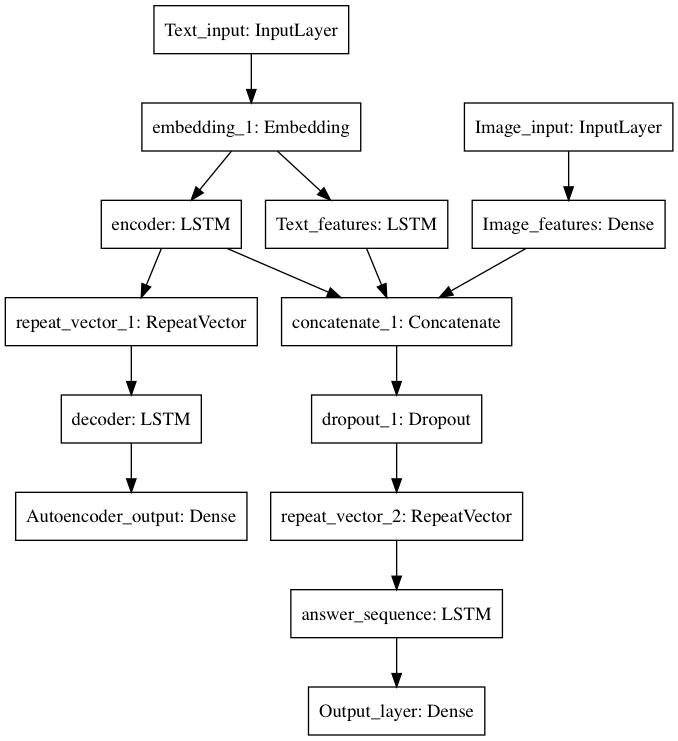
\includegraphics[scale=0.3]{classifier_w_autoencoder.png}} & 
			\subfloat[Reduced model, without autoencoder]{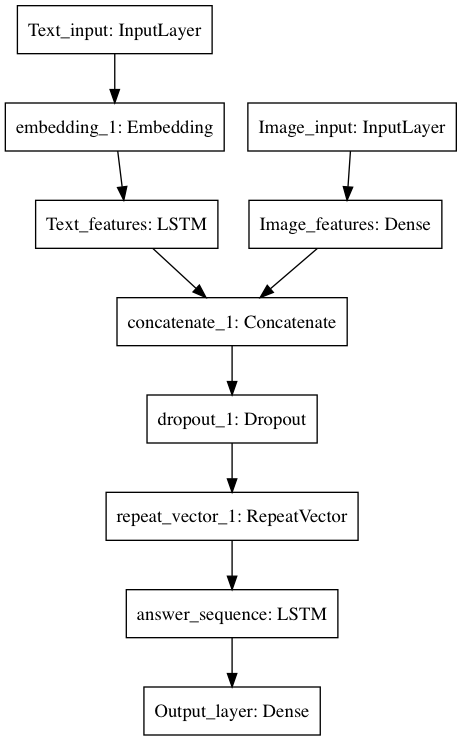
\includegraphics[scale=0.3]{classifier.png}}
		\end{tabular}
	\caption{The two different models considered in the VQA task. \label{vqa}}
	\end{figure} 
	\subsection*{Parameter choice}
	As above we tried to have a manageable number of free hyper parameters to optimize. Therefore are all LSTM layers (except the decoder) kept at the same amount of hidden neurons of 512. These could of course be individually tuned, but with the training time for the network to start performing well (sometimes 30-50 epochs), this was unpractical. The choice of optimizer and activation function in the Dense layers were also held static. For this network they are \texttt{adam} and \texttt{softmax} as these were referenced by both the general public and the literature as the best performing. The Dropout parameter had surprisingly little effect on the networks performance, and maybe should be dropped to simplify the model.
	\subsection*{Predictions}
	The accuracy of the questions are $ 15.4\% $ for the model including the autoencoder. So we can see that this model performs worse than text-only. This is a bit counter-intuitive but could be up to limited hyper parameter tuning or curse of dimensionality, even if the latter is less likely. There are also some risk of overfitting hitting our system, but that the structure is such that it's harder to detect. We did use a validation set, but it might not offer the overall accuracy we needed. The WUPS score was $ 0.205 $ with the autoencoder. If we exclude the autoencoder we can increase the performance relative to the autoencoder case. We observe an accuracy of $ 0.182 $ and WUPS score of $ 0.221 $. The paper \textit{Ask your Neurons by Mateusz Malinowski et. al.} shows that the performance of the network doesn't improve significantly when adding visual information. It's however counter-intuitive why adding the autoencoder would punish the results so significantly.  
	
	
\end{document}